Jak widzimy otrzymany wynik różni się od oczekiwanego.
Dlatego też przeprowadzimy trening sieci, którego celem będzie ustawienie wag w ten sposób,
żeby wyjście sieci jak najbardziej odpowiadało wartości oczekiwanej.

Mając obliczone wyjście sieci oraz wartością oczekiwaną możemy obliczyć wartość błędu. Robimy to przy pomocy funkcji błędu średniokwadratowego.

\[
    E(O)=1/n*(d-y)^2
\]
gdzie:
\begin{itemize}
  \item E(O) to błąd średniokwadratowy dla konkretnego neuronu wyjściowego
  \item n to liczba neuronów warstwy wyjściowej
  \item d to oczekiwane wyjście neuronu
  \item y to rzeczywiste wyjście neuronu
\end{itemize}

Suma błędów średniokwadratowych wszystkich neuronów wyjściowych jest błędem całkowitym.

\begin{figure}[!ht]
  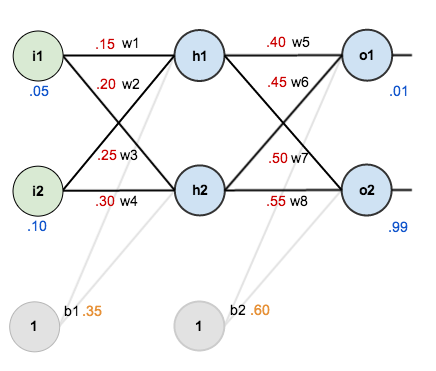
\includegraphics[width=\linewidth]{images/feed-forward-diagram-with-values.png}
  \source{https://mattmazur.com/2015/03/17/a-step-by-step-backpropagation-example/}
  \caption{Przykład wielowarstwowej sieci jednokierunkowej z podanymi wejściami oraz oczekiwanymi wyjściami}
\end{figure}

Rozważmy sieć z rysunku 2, na którym zostały podane wejścia oraz oczekiwane wyjścia sieci.
Wartości neuronów warstwy wyjściowej będą równe:
\[
    out_{o1} \approx 0.7513
\]
\[
    out_{o2} \approx 0.7729
\]
Mając podane oczekiwane oraz rzeczywiste wyjście możemy obliczyć błąd średniokwadratowy dla obu neuronów:
\[
    E_{o1} = 1/2 * (0.01-0.7513)^2 \approx 0.274762845 
\]

\[
    E_{o2} = 1/2 * (0.99-0.7729)^2 \approx 0.023566205 
\]

Tym samym błąd całkowity wynosi:
\[
    E_{total} = E_{o1}+E_{o2} \approx 0.274762845 + 0.023566205 \approx 0.29832905
\]

Jak widzimy sieć jest daleka do ideału, dlatego będziemy chcieli zmodyfikować wagi tak,
aby jak najbardziej zminimalizować błąd. Robimy to za pomocą wzoru:

\begin{gather}
  \begin{aligned}
  w_5^{+} = w_5 - \eta * \frac{\partial E_{total}}{\partial w_{5}}\\
  \end{aligned}\notag
  \shortintertext{gdzie:}
  \begin{aligned}
    &w_5^{+} ~\text{jest nową wartością wagi}.\\
    &w_5 ~\text{jest aktualną wartością wagi}.\\
    &\eta ~\text{jest stałą uczenia, czyli wartością, która określa szybkość uczenia sieci}.\\
    &\frac{\partial E_{total}}{\partial w_{5}} ~\text{jest pochodną częściową błędu całkowitego sieci do danej wagi.}
  \end{aligned}\notag
\end{gather}

Szczególną uwagę należy poświecić stałej uczenia \texteta.
Jest ona ustawiana w momencie rozpoczynania procesu, przyjmując wartości z zakresu [0,1].
W zależności od wybranej wartości, zmiany wag będą postępować gwałtowanie lub też łagodnie. 
Zazwyczaj stała uczenia jest ustawiane na wartości mniejsze od 0.1.
Jednakże w tym przykładzie ustawimy ją na 0.5.

Kolejną rzeczą wartą uwagi jest pochodna błędu całkowitego do konkretnej wagi.
Liczymy ją z wykorzystaniem reguły łańcuchowej, w przypadku \(w_5\):
\[
  \frac{\partial E_{total}}{\partial w_{5}} = \frac{\partial E_{total}}{\partial out_{o1}} * \frac{\partial out_{o1}}{\partial net_{o1}} * \frac{\partial net_{o1}}{\partial w_{5}}
\]
Już teraz możemy zauważyć, że wzór na pochodną cząstkową dla w6 będzie bardzo podobny:
\[
  \frac{\partial E_{total}}{\partial w_{6}} = \frac{\partial E_{total}}{\partial out_{o1}} * \frac{\partial out_{o1}}{\partial net_{o1}} * \frac{\partial net_{o1}}{\partial w_{6}}
\]

Wynika to z tego, że oba połączenie mają taki neuron docelowy.
Aby nie liczyć tego samego dwa razy, możemy wprowadzić oznaczenie dla części wspólnej równania:
\[
  \delta_{o1} = \frac{\partial E_{total}}{\partial net_{o1}} = \frac{\partial E_{total}}{\partial out_{o1}} * \frac{\partial out_{o1}}{\partial net_{o1}} 
\]
tym samym:
\[
  \frac{\partial E_{total}}{\partial w_{5}} = \delta_{o1}  * \frac{\partial net_{o1}}{\partial w_{5}}
\]
\[
  \frac{\partial E_{total}}{\partial w_{6}} = \delta_{o1}  * \frac{\partial net_{o1}}{\partial w_{6}}
\]

Spróbujmy teraz uprościć wyrażenie \(\frac{\partial net_{o1}}{\partial w_{5}}\):
\[
  \frac{\partial net_{o1}}{\partial w_{5}} = \frac{\partial (w_5 * out_{h1} + w_6 * out_{h2} + b_2 * 1)}{\partial w_{5}}
  = 1 * out_{h1} * w_5^{(1 - 1)} + 0 + 0 = out_{h1}
\]
Jak widzimy \(\frac{\partial net_{o1}}{\partial w_{5}}\) ostatecznie sprowadza się do wartości neuronu źródłowego dla połączenia.
W analogiczny sposób upraszcza się równanie dla \(\frac{\partial net_{o1}}{\partial w_{6}}\), dzięki czemu otrzymujemy:
\[
  \frac{\partial E_{total}}{\partial w_{5}} = \delta_{o1}  * out_{h1}
\]
\[
  \frac{\partial E_{total}}{\partial w_{6}} = \delta_{o1}  * out_{h2}
\]

Ostatnim krokiem potrzebnym do wyliczenia nowych wag \(w_5\) jest obliczenie samego współczynnika delty dla \(o_1\) (\(\delta_{o1}\)):

\[
  \delta_{o1} = \frac{\partial E_{total}}{\partial net_{o1}} = \frac{\partial E_{total}}{\partial out_{o1}} * \frac{\partial out_{o1}}{\partial net_{o1}}
\]

\begin{gather}
  \begin{aligned}
    &\frac{\partial E_{total}}{\partial out_{o1}} = \frac{\partial (\frac{1}{2}(d_{o1} - out_{o1})^{2} + \frac{1}{2}(d_{o2} - out_{o2})^{2})}{\partial out_{o1}}
  \end{aligned}\\
  \begin{aligned}\\
    &= 2 * \frac{1}{2}(target_{o1} - out_{o1})^{2 - 1} * -1 + 0 \\
  \end{aligned}\\
  \begin{aligned}
    &= -(target_{o1} - out_{o1}) \\
  \end{aligned}
\end{gather}

\begin{gather}
  \begin{aligned}
    &\frac{\partial out_{o1}}{\partial net_{o1}} =  \frac{\partial (\frac{1}{1+e^{-net_{o1}}})}{\partial net_{o1}}
  \end{aligned}\\
  \begin{aligned}\\
    &=({\frac{1}{1+e^{-net_{o1}}})}(1 - \frac{1}{1+e^{-net_{o1}}}) \\
  \end{aligned}\\
  \shortintertext{gdzie:}
  \begin{aligned}
    \frac{1}{1+e^{-net_{o1}}}=out_o1
  \end{aligned}
  \shortintertext{a więc:}
  \begin{aligned}
    \frac{\partial out_{o1}}{\partial net_{o1}} = out_{o1}(1 - out_{o1})
  \end{aligned}
\end{gather}

W związku z powyższymi równaniami wzór na współczynnik delty dla \(out_o1\) wynosi:

\begin{gather}
  \begin{aligned}
    \delta_{o1} = \frac{\partial E_{total}}{\partial net_{o1}} = \frac{\partial E_{total}}{\partial out_{o1}} * \frac{\partial out_{o1}}{\partial net_{o1}}
  \end{aligned}\\
  \begin{aligned}\\
    &= -(target_{o1} - out_{o1}) * out_{o1}(1 - out_{o1}) \\
  \end{aligned}\\
\end{gather}


\begin{gather}
  \begin{aligned}
    \delta_{o1} = \frac{\partial E_{total}}{\partial net_{o1}} = \frac{\partial E_{total}}{\partial out_{o1}} * \frac{\partial out_{o1}}{\partial net_{o1}}
  \end{aligned}\\
  \begin{aligned}\\
    &= -(target_{o1} - out_{o1}) * out_{o1}(1 - out_{o1}) \\
  \end{aligned}\\
\end{gather}

Co podstawieniu daje:
\[
  \frac{\partial E_{total}}{\partial w_{5}} = \delta_{o1}  * out_{h1} = -(target_{o1} - out_{o1}) * out_{o1}(1 - out_{o1}) \approx 0.1385
\]

W ten sposób otrzymaliśmy łatwy wzór na obliczenie pochodnych cząstkowej po w5 i w6
\[
  \frac{\partial E_{total}}{\partial w_{5}} = \delta_{o1}  * out_{h1} \approx  0.1385 * 0.593269992 \approx 0.082167
\]
\[
  \frac{\partial E_{total}}{\partial w_{6}} = \delta_{o1}  * out_{h2} \approx  0.1385 * 0.596884378 \approx 0.082668
\]

co umożliwia nam obliczenie nowych wag:
\[
  w_5^{+} = w_5 - \eta * \frac{\partial E_{total}}{\partial w_{5}} = 0.4 - 0.5 * 0.082167 = 0.359
\]
\[
  w_6^{+} = w_6 - \eta * \frac{\partial E_{total}}{\partial w_{6}} = 0.45 - 0.5 * 0.082668 = 0.409
\]

W analogiczny sposób liczymy nowe wagi połączeń z neuronem \(o_2\):
\[
  w_7^{+} = w_7 - \eta * \frac{\partial E_{total}}{\partial w_{7}} = w_7 - \eta * \delta_{o2}  * out_{h1} = 0.511
\]
\[
  w_8^{+} = w_8 - \eta * \frac{\partial E_{total}}{\partial w_{8}} = w_8 - \eta * \delta_{o2}  * out_{h2} = 0.561
\]

Bias jest trochę innych w przypadkiem, gdyż jest połączony jednocześnie z neuronami o1 i o2, w związku z tym pochodna cząstkowa do tej wagi będzie wyliczana w następujący sposób:

\begin{gather}
  \begin{aligned}
    \frac{\partial E_{total}}{\partial b_2} = \frac{\partial E_1+E_2}{\partial b_2}=\frac{\partial E_1}{\partial b_2}+\frac{\partial E_2}{\partial b_2}
  \end{aligned}\\
  \begin{aligned}\\
    = (\frac{\partial E_1}{\partial b_2})
  \end{aligned}\\
\end{gather}


\[
  b_2^{+} = b_2 - \eta * \frac{\partial E_{total}}{\partial b_2} = b_2 - \eta * \delta_{o1}+\delta_{o_2}  * out_{h2} = 0.561370121
\]









